\section{Data Summary \& Motivation}  \label{sec:features}

\begin{figure}
    \centering
    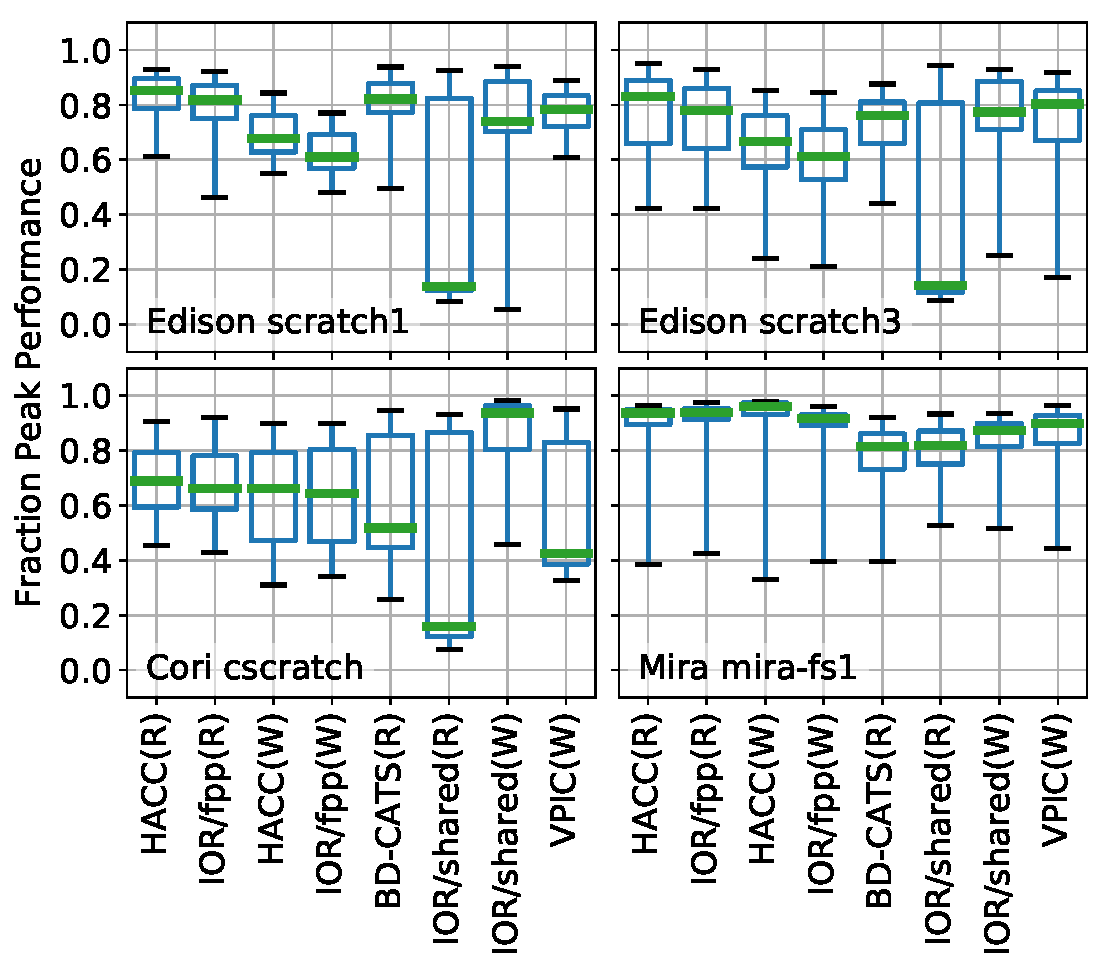
\includegraphics[width=0.9\columnwidth]{summary-boxplots}
    \vspace{-.15in}
    \caption{I/O performance grouped by test applications and read(R)/write(W) mode.  Whiskers represent the 5th and 95th percentiles.}
    \label{fig:summary-boxplots}
%   \vspace{-.3in}
\end{figure}


\begin{figure*}
    \centering
    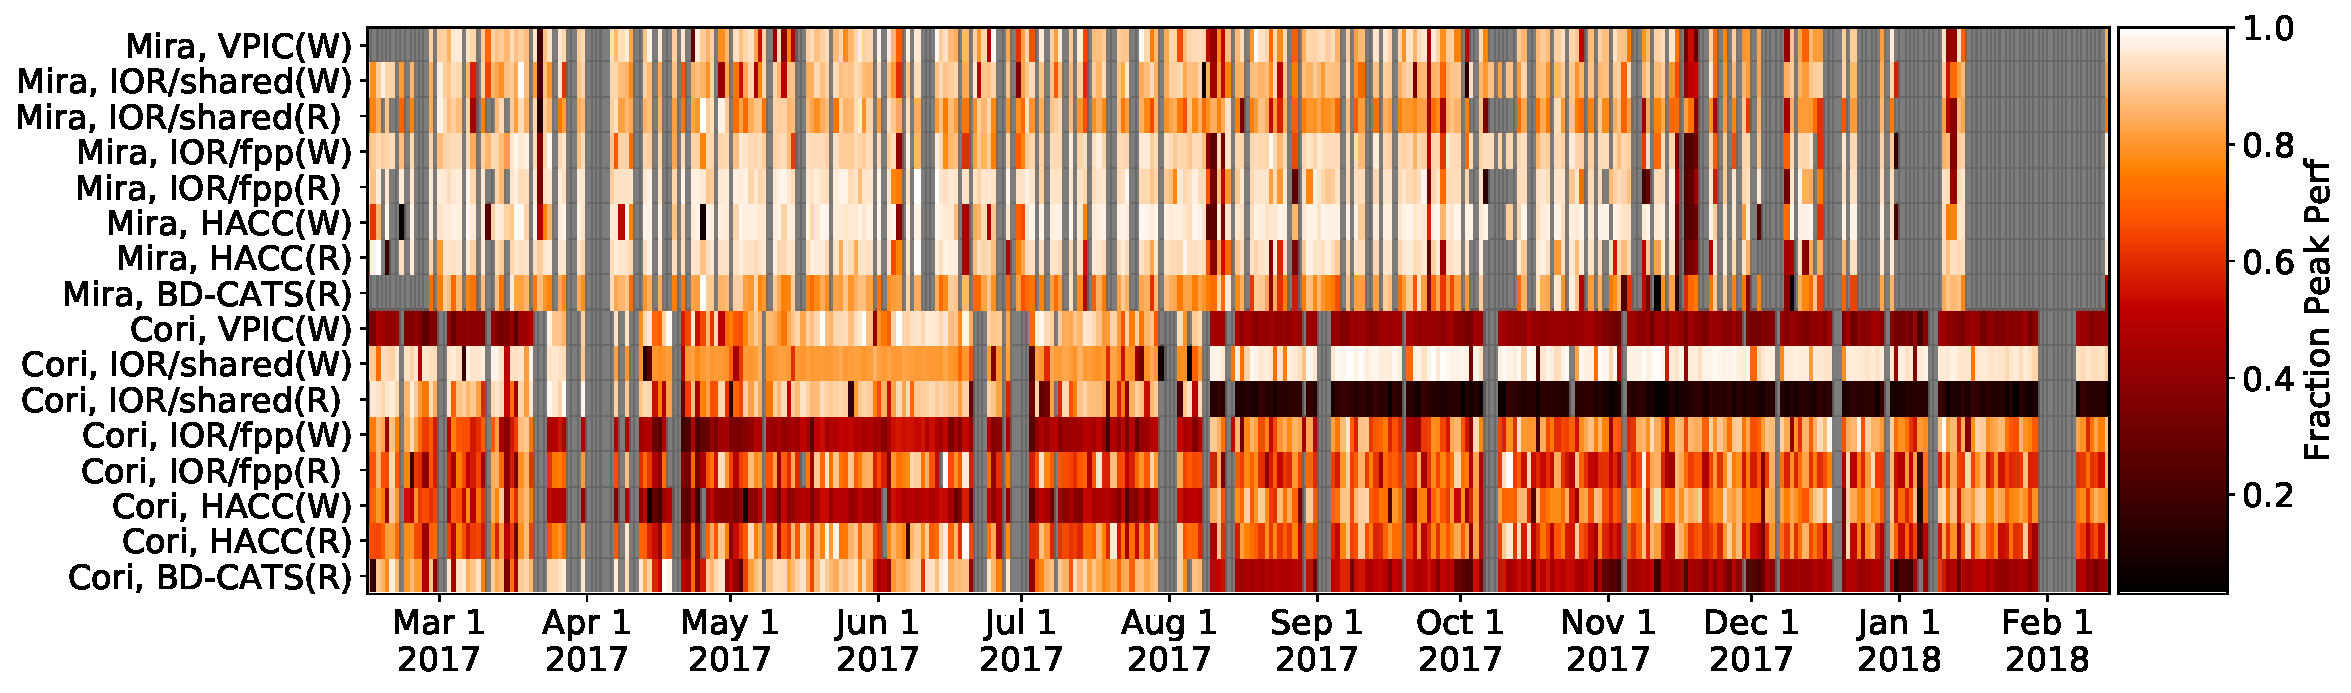
\includegraphics[width=0.90\linewidth]{summary-heatmap}
    \vspace{-.2in}
    \caption{Performance of daily benchmarks normalized to each benchmark's peak observed performance on the specified storage system.  The y-axis labels show combinations of system, I/O motif, and mode (Read/Write).  Grey represents days on which no observations were made.  The two regions highlighted in green boxes are expanded upon in Figure \ref{fig:regions-heatmap}.}
    \label{fig:summary-heatmap}
\end{figure*}

\begin{figure}
    \centering
    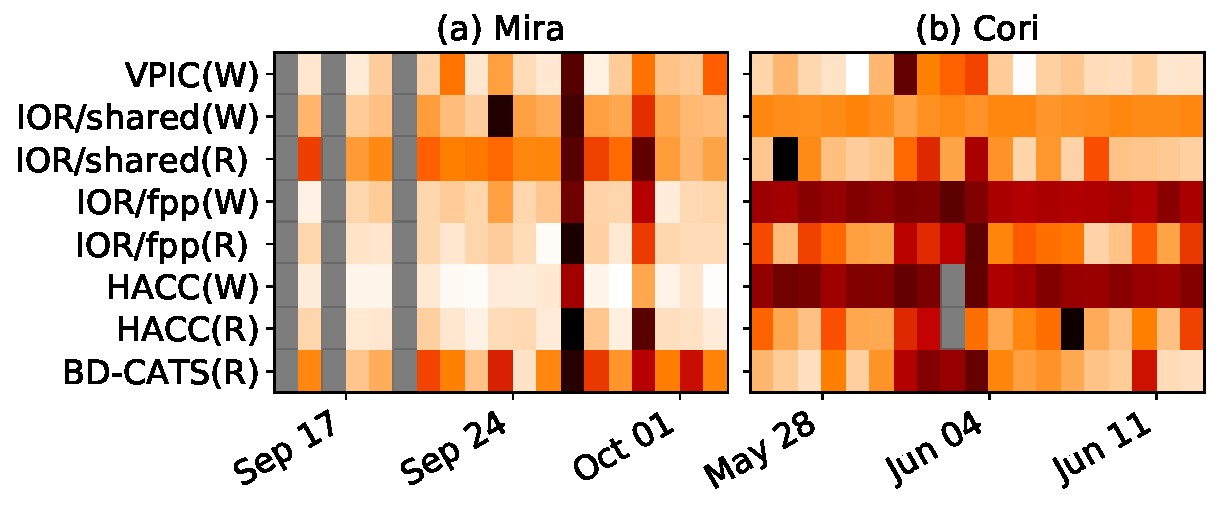
\includegraphics[width=0.90\linewidth]{regions-heatmap}
    \vspace{-.2in}
    \caption{Examples of structure in the fraction of peak performance observations.  Color scale is the same as that in Figure \ref{fig:summary-heatmap}.  In (a), the vertical band on Sept 26 corresponds to a transient system-wide degradation on \mira.  The horizontal bands for the IOR file-per-process write workload (IOR/fpp(W)) and HACC write workload (HACC(W)) in (b) show a sustained performance problem for file-per-process write workloads on \cori.}
    \label{fig:regions-heatmap}
\end{figure}

\subsection{Statistical overview} \label{sec:features/summary}

% \TODO{Things that are important here: behavior over time, grouping data sources in a way that helps understand scope, focusing on fundamental \emph{changes} in performance rather than steady state, everything in one view.}

I/O performance is known to vary as a function of (a) application I/O pattern, (b) whether I/Os read or write, and (c) the architecture of the system on which I/O is happening~\cite{Lockwood2017, Xie2012}.
To remove the effects of these factors and enable us to focus on performance \emph{variation}, we express the performance of each of the 11,986 observations in terms of its \emph{fraction of peak performance}.
This fraction of peak performance is defined as the absolute performance (in bytes/sec) of an observation divided by the maximum absolute performance observed across all jobs with a common (a), (b), and (c) above.

The distribution of the fraction of peak performance measurements for four of the five systems tested is shown in Fig. \ref{fig:summary-boxplots} and demonstrates that the performance of active I/O performance probes on production file systems is highly dynamic.
However, visualizing the raw data of two of these performance distributions (Fig. \ref{fig:summary-heatmap}) reveals that performance variation is not randomly distributed over the year, and time-independent distributions of performance variation do not fully capture the nature of performance variability in production storage systems.
Several archetypical types of correlated performance degradation observed in Fig. \ref{fig:summary-heatmap} are highlighted in Fig. \ref{fig:summary-heatmap} and fall into three broad categories of variation:

\begin{enumerate}[leftmargin=*]
\item Dark vertical bands, exemplified in the \mira data in Fig. \ref{fig:regions-heatmap}, represent transient system-wide issues that resulted in a uniform loss of performance for all applications tested that day.
\item Dark horizontal bands, shown in the \cori data, indicate a long-term degradation in performance that disproportionately affects a specific I/O motif or reads or writes.
\item Isolated dark blocks represent individual application runs where performance was poor for a very short period of time within a day.
\end{enumerate}

% - Baseline performance and variability are not constant over time.  Predictive models must therefore adapt over time as well.
The preponderance of these time-dependent phenomena underscore the observation that \textbf{baseline I/O performance and variability are not constant over time}, and
what may qualify as abnormally poor performance during one period of time may be the baseline performance expectation during another.

This has implications for both HPC operators and users.
For system architects and operators, identifying and remedying the root causes of variation requires classifying an absolute performance measurement with respect to the performance region in which it was observed to determine if it was the result of a long-term divergence from baseline peak performance or if it was caused by a transient issue in the system.
% From Phil: In the prose we can site several predictive model papers (Bing Xie's papers, Sandeep's papers, and others) and point out that the implication is that these models aren't just "set it and forget it."  Not knocking them or even saying they can't do it, but just pointing out it's not covered yet.
For users and application developers, it follows that the accuracy of parameterized I/O performance models~\cite{Xie2012,Madireddy2017} will degrade unless they are reparameterized as the I/O subsystem they model evolves.
Both of these cases justify the need for a systematic approach for identifying different regions of I/O performance to differentiate long-term factors and phenomena from short-term transients.

\subsection{Time-dependent analysis} \label{sec:features/timedependent}

\begin{figure}[t]
    \centering
    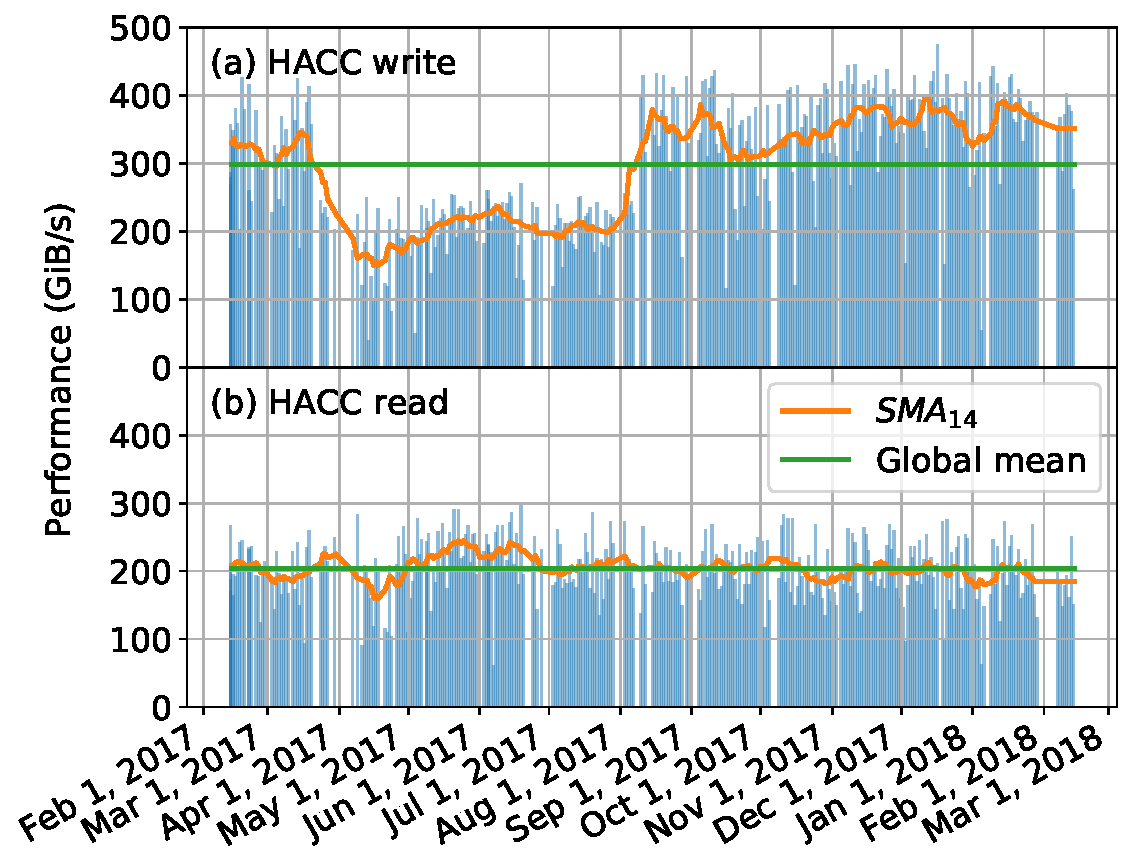
\includegraphics[width=1.0\columnwidth]{longterm-cscratch-hacc}
    \vspace{-.35in}
    \caption{Performance evolution of HACC file-per-process workload on \cori.  Red line is the overall mean (298 GiB/sec write, 204 GiB/sec read) and blue bars are raw performance measurements.}
    \label{fig:timeseries-baseline}
    % source: sc18_segments.ipynb
\end{figure}




% \begin{figure}[t]
%     \centering
%     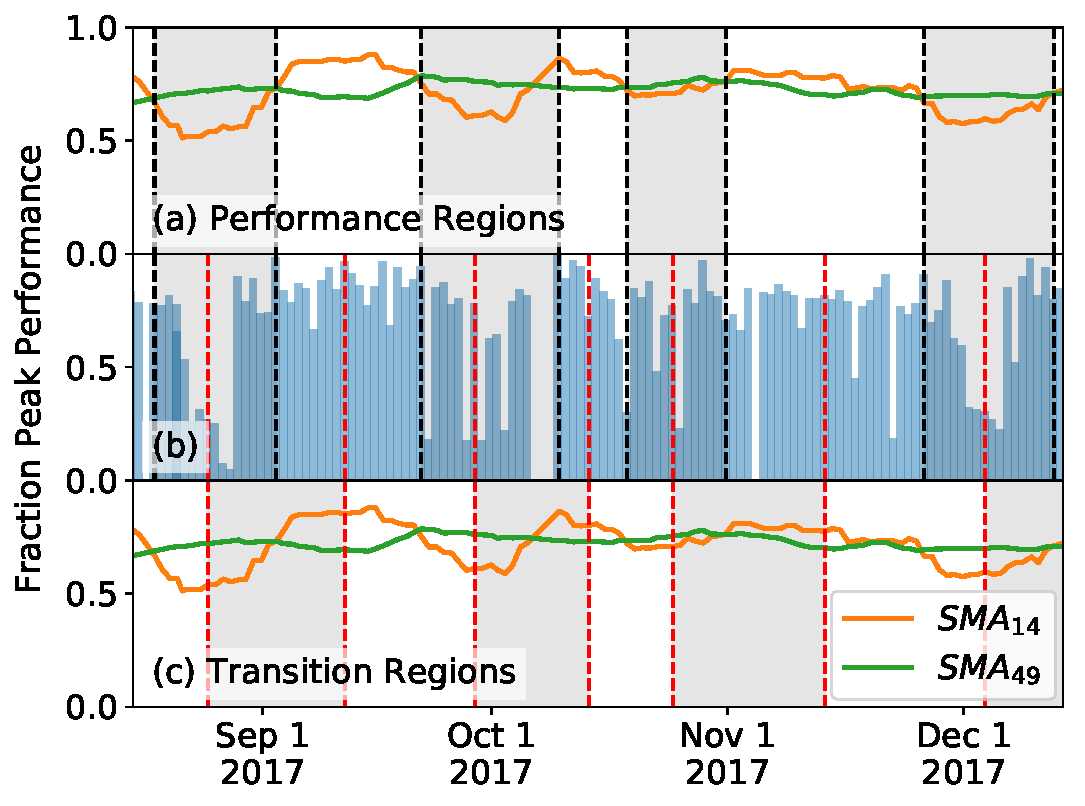
\includegraphics[width=1.0\columnwidth]{segment-explain}
%     \vspace{-.35in}
%     \caption{Example of overlaying two simple moving averages (SMAs) to identify (a) \emph{divergence regions} and (c) \emph{trend regions} in the \edison \scratchtwo IOR/fpp write dataset.  Middle pane (b) includes raw performance measurements (blue bars) with both SMA crossovers (black dashed lines) and divergence region centroids (red dashed lines).}
%     \label{fig:segment-explain}
    % source: sc18_segments-explain.ipynb
% \end{figure}

To address this need for systematic partitioning of performance regions, we propose applying Simple Moving Averages (SMAs) to the data collected from active I/O performance.
Given a time window of width $w$, the SMA for performance at time $t$ as the arithmetic mean of the fraction peak performance over ${-0.5w <= t < +0.5w}$.
When chosen to be sufficiently short (${w_{short} \sim O(\textup{days})}$), the resulting $\textup{SMA}_{short}$ provides a rapid visual means to identify performance degradation or recovery that lasts for $O(\textup{days})$.







Superimposing a second SMA with a longer window ($\textup{SMA}_{long}$, where ${w_{short} \sim O(\textup{weeks})}$) then allows us to compare short-term performance variations to the longer-term average, effectively distinguishing anomalies that last for $O(\textup{days})$ from longer-term performance evolution that occurs over $O(\textup{weeks})$.
The points at which $\textup{SMA}_{short}$ intersects $\textup{SMA}_{long}$, termed \emph{crossover points}, also conveniently establish the boundaries of regions where short-term performance has diverged from longer-term performance.

We borrow this approach from financial market technical analysis, where moving averages are used to attenuate the day-to-day volatility in price movements and help identify larger trends in the price of different underlying assets~\cite{james1968monthly,gunasekarage2001profitability}.
SMA crossover points are, again, a popular tool in technical analysis of financial markets, used to detect trend shifts in asset prices, often for predictive purposes\footnote{Though we note that the predictive capability of SMA crossovers is a source of controversy even in the financial community, and thus, we focus solely on using them as tools for managing volatility and detecting trends in historical datasets.} (e.g., as signals to buy or sell an asset based on the direction of the short and long-term SMAs at the time they crossover)~\cite{brock1992simple}.



% In the following analysis, we apply this SMA-based approach to procedurally identify and classify performance variation at all time scales, ranging from long-term system health issues to transient performance loss due to probabilistic contention.


%We define $\textup{SMA}_{short}$ and $\textup{SMA}_{long}$ as simple moving averages of widths $w_{short}$ and $w_{long}$, and for this study, chose $w_{short} = 14$ days and $w_{long} = 49$ days as a reasonable choice to focus on correlated performance events that occurred over $O(\textup{weeks})$.

% J_{app, rw, sys}


After calculating $\textup{SMA}_{short}$ and $\textup{SMA}_{long}$ for each of the set of performance observations $J_{app, rw, sys}$, we identify \emph{divergence regions}. These are defined as non-overlapping subsets of $J_{app, rw, sys}$ that are bounded by the crossover points between $\textup{SMA}_{long}$ and $\textup{SMA}_{short}$.




%Figure \ref{fig:segment-explain}a illustrates this partitioning of the IOR/fpp write workload measurements on \edison's \scratchtwo file system;
%dashed lines represent the crossover points of $\textup{SMA}_{long}$ and $\textup{SMA}_{short}$, and divergence regions are shaded in alternating gray and white.
%As Figure \ref{fig:segment-explain}a illustrates, using SMA crossovers to identify divergence regions results in temporally contiguous subsets of performance measurements that capture a period of time with consistently good (${\textup{SMA}_{short} > \textup{SMA}_{long}}$) or bad (${\textup{SMA}_{short} < \textup{SMA}_{long}}$) performance.

%Figure~\ref{fig:segment-explain}a shows 8 distinct divergence regions, but does not provide any insight into the causes of the transitions. To understand the causes of these transitions, we also partition $J_{app, rw, sys}$ into \emph{trend regions}.
%For each divergence region, we identify the temporally center-most observation as the centroid of that region, as illustrated in Figure \ref{fig:segment-explain}b, as red dashed lines.
%We then define trend regions as those regions bounded by centroids (Figure \ref{fig:segment-explain}c), and each trend region overlaps with exactly two divergence regions and vice versa.
%The principal difference between the two is that divergence regions contain observations that are uniformly good or uniformly bad, and trend regions capture performance transitioning from bad to good or vice versa. Divergence regions are used to group measurements which are similar, trend regions are used to understand the reasons for transition between different performance regimes.

%\TODO{Can we say more here about what we learned from Figure 3?}


